\documentclass[webpdf,modern,large]{biorxiv}
\usepackage[a4paper,top=25mm,bottom=25mm,left=17.5mm,right=17.5mm]{geometry}

\graphicspath{{Fig/}}


\usepackage{booktabs}   % Improves table formatting
\usepackage{array}      % For better table formatting
\usepackage{makecell}
\usepackage[T1]{fontenc}
\usepackage[english]{babel}
\usepackage{microtype}
\usepackage{hyperref}
\usepackage{url}

\providecommand{\doi}[1]{\href{https://doi.org/#1}{doi:\nolinkurl{#1}}}

\hyphenpenalty=1000
\exhyphenpenalty=1000


\begin{document}

\copyrightyear{2026}

\firstpage{1}

\title[Benchmarking long-read simulators against Oxford Nanopore whole-genome sequencing data]{Benchmarking long-read simulators against Oxford Nanopore whole-genome sequencing data}

\author[1]{Mona L Taouk\ORCID{0000-0003-3820-5338}}
\author[1,2,$\dagger$,$\ast$]{Danielle J Ingle\ORCID{0000-0003-0707-6537}}
\author[1,2,$\dagger$,$\ast$]{Ryan R Wick\ORCID{0000-0001-8349-0778}}

\authormark{Taouk et al.}

\address[1]{\orgdiv{Department of Microbiology and Immunology}, \orgname{The University of Melbourne at the Peter Doherty Institute for Infection and Immunity}, \orgaddress{Melbourne, Victoria, Australia}}
\address[2]{\orgdiv{Centre for Pathogen Genomics}, \orgname{The University of Melbourne}, \orgaddress{Parkville, Victoria, Australia}}

\corresp[$\dagger$]{These authors contributed equally\\}

\corresp[$\ast$]{Corresponding authors:
\href{mailto:danielle.ingle@unimelb.edu.au}{danielle.ingle@unimelb.edu.au},
\href{mailto:ryan.wick@unimelb.edu.au}{ryan.wick@unimelb.edu.au}}




\abstract{
\textbf{Background:}
Oxford Nanopore Technologies (ONT) sequencing is increasingly used for whole-genome sequencing (WGS) across a wide range of applications. However, the platform has evolved rapidly through updates to flow cell chemistry and basecalling algorithms, altering the characteristics of the resulting sequencing data. Read simulators provide synthetic datasets with known ground truth, enabling controlled development and evaluation of methods. However, many existing simulators were developed for earlier versions of ONT sequencing or use generic long-read assumptions, and their realism for contemporary ONT data is unclear.
\vspace{0.5\baselineskip}\\
\textbf{Results:}
We benchmarked six ONT-compatible read simulators (Badread, LongISLND, lrsim, NanoSim, PBSIM3 and SimLoRD) using a microbial genome reference and ONT R10.4.1 reads as the empirical standard. Each tool was configured to maximise realism, including training on empirical reads when supported. We compared simulated and real datasets with respect to read length, read accuracy, FASTQ quality scores and sequence error profiles. No simulator reproduced all metrics of the real data well. PBSIM3 most closely reproduced read accuracy and FASTQ quality scores, making it a strong simulator for broad read-level realism. However, it did not capture important features of the real error profile, including context-dependent substitution rates and homopolymer-length errors. Badread and LongISLND better reproduced some aspects of the error profile, but showed other departures from the real data.
\vspace{0.5\baselineskip}\\
\textbf{Conclusion:}
PBSIM3 is a good general-purpose choice for many ONT WGS microbial simulation tasks because it reproduced several key read-level properties well. However, Badread or LongISLND may be preferable for applications where error structure is more important. No evaluated tool was realistic across all tested metrics, highlighting a gap for improved long-read simulators.
}

\keywords{Oxford Nanopore, long-read sequencing, read simulators, benchmarking, sequencing errors}



\maketitle



\section{Background}

Oxford Nanopore Technologies (ONT) sequencing has transformed long-read genomics by enabling real-time, portable and increasingly high-throughput sequencing\cite{jain2016oxford}. Over the past decade, ONT platforms have changed rapidly, particularly through updates to nanopore chemistry and basecalling models\cite{OxfordNanopore2024,wick2019performance}. Consequently, the characteristics of ONT data, such as error profiles and base quality scores (Q-scores), have shifted substantially over relatively short time frames of a few years\cite{rang2018squiggle,wang2021nanopore}. ONT benchmarking studies can age quickly, because their conclusions depend on the chemistries, protocols and basecalling models available at the time\cite{bogaerts2024closing}. Although ONT continues to evolve, recent changes in read accuracy are now more gradual than the major advances seen earlier in the platform's development. This increasing stability is making ONT more attractive for routine, high-throughput applications where analytical pipelines must withstand formal validation and accreditation\cite{mostafa2024evolution,sereika2022oxford}.

As ONT sequencing matures, its use is expanding both in high-income countries, where laboratories are now more willing to invest in validation of ONT-based workflows, and in low- and middle-income settings, where ONT's low capital cost and portability make it a compelling alternative to some short-read sequencers\cite{avershina2022ultrafast, moso2024non, sheka2021oxford}. In both contexts, there is a need for robust, realistic benchmarking of long-read analysis tools for tasks such as read mapping, variant calling and genome assembly\cite{wick2025autocycler, sovic2016fast, cretu2017mapping}. Benchmarking using real ONT datasets is essential, but it is also constrained by sample availability, cost and the difficulty of establishing a ground truth, particularly for complex genomes\cite{wick2025autocycler}. Read simulators therefore play an important role: they provide synthetic datasets where the underlying sequence is exactly known, enabling controlled, reproducible evaluation of methods across a range of experimental designs. They can also supply the large labelled training sets needed for machine learning methods such as deep neural networks\cite{vrcek2025}.

However, many widely used ONT-compatible simulators were originally developed for earlier generations of ONT (pre-R10.4.1 flowcells) or PacBio long-read sequencing, and they may incorporate assumptions that no longer hold for modern ONT\cite{yang2017nanosim, ono2022pbsim3, wick2019badread, lau2016longislnd, stocker2016simlord}. For example, simulators often assumed high error rates and a simple error structure\cite{yang2017nanosim, wick2019badread}. Since then, improvements in ONT chemistry and basecalling have improved read accuracy, altered the balance between substitutions and indels, and changed the relationship between FASTQ Q-scores and error rates\cite{sereika2022oxford}. It is therefore unclear whether existing simulators can produce reads that resemble contemporary ONT data.

ONT simulators differ fundamentally in how they generate reads. Some tools rely on explicit training with real data, learning an empirical error model by aligning ONT reads to a reference genome and then using it to introduce errors into new sequences\cite{lau2016longislnd, ono2022pbsim3, yang2017nanosim}. Others use pre-trained models that encapsulate typical error behaviour for a given technology and chemistry. Others generate reads from parametric distributions specified by the user, without direct training on empirical data\cite{wick2019badread, stocker2016simlord}. These design choices affect not only how realistic the resulting reads are for a given technology snapshot, but also how easily the simulator can be adapted as ONT chemistries and basecalling models evolve. In particular, simulators that train an error profile from alignments of real reads to a reference have the potential to adapt to new read types.

In this context, `realism' refers to how closely simulated reads resemble real ONT data across multiple dimensions that matter for downstream analysis. These include basic read-level metrics, such as the distributions of read length, read accuracy and FASTQ Q-scores, together with relationships between these metrics and finer-scale error profiles. The primary goal of this study is therefore to evaluate which currently available read simulators produce the most realistic data for modern ONT reads, focusing on faithfulness to empirical read characteristics.




\section{Methods}

\subsection{Simulator selection}
A literature search identified seven long‑read simulators compatible with ONT reads. SimON‑reads\cite{simonreads} was excluded because it failed to produce reads under any of the specified configuration flags and was deemed non‑functional for this analysis. The other six simulators were successfully evaluated in this study: Badread v0.4.2\cite{wick2019badread}, LongISLND v0.9.5 (\texttt{c458f56})\cite{lau2016longislnd}, lrsim v0.7\cite{lrsim}, NanoSim v3.2.3\cite{yang2017nanosim}, PBSIM3 v3.0.5\cite{ono2022pbsim3}, and SimLoRD v1.0.4\cite{stocker2016simlord}.


\subsection{Reference data}
Real ONT reads used as the empirical benchmark were generated from \textit{Listeria innocua} strain AUSMDU00097349 (accession \href{https://www.ncbi.nlm.nih.gov/biosample/SAMN46906078}{SAMN46906078}) on an ONT R10.4.1 PromethION flow cell and basecalled with Dorado v1.1.1\cite{dorado} using the \texttt{dna\_r10.4.1\_e8.2\_400bps\_sup@v5.2.0} basecalling model, the latest available for this chemistry at the time of analysis. Reads were demultiplexed using the \texttt{dorado demux} with default parameters using the built-in \texttt{SQK-RBK114-96} kit barcodes, and reads assigned to barcode 5 (corresponding to the \textit{L. innocua} sample) were retained. The demultiplexing step incidentally excludes some poor-quality reads with absent or unrecognisable barcodes, but no explicit Q-score or length filtering was applied.

The real read set comprised 680,482 reads with a total length of 3,803 Mbp, mean length of 5,588 bp and N50 length of 8,923 bp. The reads were split into two non-overlapping sets: a test set of 53,093 randomly selected reads (chosen to total 100$\times$ depth) and a training set containing the remaining 627,389 reads. The test set was used to evaluate real-read properties, while the training set was used to train simulators.

Simulated reads were generated from a complete, closed assembly of the same \textit{L. innocua} strain. This 2,972,545 bp genome was produced in a previous study from the same ONT read set, with Illumina reads used for polishing \cite{wick2025autocycler}. Because the assembly was carefully resolved and polished, it provided a reliable ground truth for both read simulation and read evaluation.


\subsection{Simulator configuration}
Each simulator was configured to maximise the realism of generated reads. For simulators with explicit training or model-building steps (Badread, LongISLND, lrsim and NanoSim), models were built from the real read training set, using alignments to the reference genome where required. PBSIM3 was run in its sampling mode, using real training reads as the source of read lengths and FASTQ quality strings, and SimLoRD was configured to sample read lengths from the training reads. For options controlling overall error rate, error variability or error-type ratios, we used values estimated from the training reads. For NanoSim and PBSIM3, we tested various homopolymer modelling options (Figures \ref{fig:supp_nanosim_homopolymers} and \ref{fig:supp_pbsim3_homopolymers}) and used the settings which best matched the real reads: disabled homopolymer length simulation in NanoSim, and \texttt{-{}-hp-del-bias 5} in PBSIM3. All tools were set to generate read sets of 100$\times$ depth ($\sim$300 Mbp).

Each simulator tool was run through GNU Time to quantify its time to run. For tools with separate training and simulation steps, these were measured separately. lrsim (simulation step) and NanoSim support multithreading and were run using 16 threads. Badread, LongISLND, lrsim (training step), PBSIM3 and SimLoRD do not support multithreading and were therefore run with one thread.

Exact commands are documented in Supplementary Methods (methods.md) and are publicly available in the \href{https://github.com/mtaouk/ONT-Read-Simulator-Benchmarking}{accompanying GitHub repository}.


\subsection{Evaluation metrics}
Simulated and real test reads were compared across multiple read-level and base-level metrics to assess realism. We did not rely on formal statistical tests, because with datasets of this size, even trivial differences can be statistically significant. Instead, we compared the shapes of distributions and the relationships between variables in simulated and real data, which provides a more direct and interpretable measure of realism. We quantified discrepancies in read-length and Q-score distributions using the Wasserstein-1 distance, calculated as the integral of the absolute difference between their normalised weighted cumulative distribution functions (Table \ref{tab:supp_distance_metrics}).

Read lengths were extracted from FASTQ files and summarised using seqkit v2.13.0\cite{shen2016seqkit}. Read length distributions were visualised as histograms using the same bin widths and axis limits across all datasets to enable direct visual comparison.

Real and simulated reads were aligned to the reference genome using minimap2 v2.30\cite{li2018minimap2}. Secondary alignments were removed, and identity was then calculated as the number of matching bases divided by the alignment length. This is the ``BLAST identity'' approach to measuring sequence similarity, where the impact of insertions and deletions is proportional to their length (e.g. a 5-bp deletion affects identity the same as five 1-bp deletions)\cite{li2018identity}. Empirical read Q-scores were computed as $Q = -10 \times \log_{10}(1 - \text{identity})$ for each read. Reported read Q-scores were calculated by converting each Phred-scaled quality value in the FASTQ file to an error probability, averaging those probabilities across the aligned portion of the read and then converting back to a Q-score.

To examine FASTQ Q-scores at the per-base level, each base was classified from the alignment as a match, mismatch or insertion, then grouped by its reported FASTQ Q-score. Because deletions have no corresponding read base and therefore no Q-score, they were represented indirectly by adjacent matching bases counted at half weight. For each reported Q-score, we then calculated the observed error rate from the counts of mismatches, insertions and deletion-associated bases, and used these values to generate calibration plots.

To characterise the error profiles of the real and simulated reads, we analysed two specific error types: 3-mer substitutions and homopolymer lengths. For 3-mer substitutions, we counted substitutions on the sequenced strand in which the middle base differed and the immediate flanking bases matched, for which there are 192 possibilities. The rate of each was expressed as the number of observed substitutions divided by the number of occurrences of the reference 3-mer in the aligned sequence. Homopolymer lengths of 3--10 bp were assessed using Pomoxis v0.3.16\cite{pomoxis}, and we defined error rate as the fraction of homopolymers in reads with an incorrect length. These analyses were not intended to capture all aspects of ONT sequencing errors, but instead provide two targeted, interpretable and directly comparable measures of error realism.

To examine how well simulated reads assemble, we generated random subsets of each test read set ranging from 1$\times$ to 50$\times$ depth, in 1$\times$ increments. Each read set was assembled using Flye v2.9.6\cite{kolmogorov2019assembly}, metaMDBG v1.4\cite{benoit2026high}, miniasm v0.3\cite{li2016minimap} plus Minipolish v0.2.1, Myloasm v0.7.0\cite{shaw2026high} and Raven v1.8.3\cite{vaser2021time}. All assemblies were run via the helper command in Autocycler v0.8.0\cite{wick2025autocycler}. For assemblies that produced at least a 2 Mbp contig ($\sim2/3$ of the genome size), assembly accuracy was quantified using the longest contig's alignment identity to the reference genome.



\section{Results}

\subsection{Characteristics of real ONT reads}

The real ONT reads had a mean empirical read Q-score of 19.0 and a mean reported read Q-score of 19.2 (Table \ref{tab:supp_read_accuracy}). Read errors were 40.1\% substitutions, 18.9\% insertions and 41.0\% deletions. The 3-mer substitution rates ranged from 0.0059\% for \texttt{CTG}→\texttt{CGG} to 3.6\% for \texttt{CGA}→\texttt{CAA}. Indel errors were especially common in longer homopolymers, with 9-bp homopolymers containing an error 35.6\% of the time.

The per-base reported Q-scores ranged from 1 (predicted error rate of 79.4\%) to 50 (predicted error rate of 0.001\% ). At a per-base level, these reported Q-scores were not perfectly calibrated, e.g. Q50 bases were incorrect (or associated with an adjacent deletion) 0.0157\% of the time, equivalent to Q38. However, at the whole-read level (averaging all bases), reported and empirical Q-scores generally showed good agreement.

In this study, we did not apply a quality-based filter to the real reads, retaining all reads produced by the basecaller. This revealed a distinctive bimodal distribution in both empirical and reported Q-scores, with a small peak at $\sim$Q8 and a larger peak at $\sim$Q23. Bimodal distributions of read Q-scores have been previously observed in ONT datasets\cite{formenti2025evaluation}, but the lower peak may be absent from quality-filtered ONT datasets, e.g. those restricted to reads classified as ``PASS'' by ONT's MinKNOW software.


\subsection{Simulator design and training strategies}

The six evaluated read simulators (Badread, LongISLND, lrsim, NanoSim, PBSIM3 and SimLoRD) differ in how they model read length, sequence errors and Q-scores (Table~\ref{tab:simulators})\cite{wick2019badread, lau2016longislnd, lrsim, yang2017nanosim, ono2022pbsim3, stocker2016simlord}. Badread uses parametric read length and identity distributions, with trained \textit{k}-mer error and Q-score models. LongISLND uses a non-parametric model that samples bases and Q-scores from training reads with matching extended-\textit{k}-mer contexts. lrsim uses a model derived from alignment statistics for read lengths and indel-size structure, with user-specified overall error parameters. NanoSim fits read length, alignment, Q-score and error distributions from aligned reads, using Markov models for error structure. PBSIM3 was run in sample mode, where it copies read lengths and Q-score strings from real reads and uses a user-specified error-type ratio. SimLoRD is based on a PacBio circular consensus sequencing (CCS) pass-count model; in this study, we disabled CCS-style behaviour to better approximate ONT sequencing, sampled read lengths from the training reads and supplied error parameters manually.

\begin{table*}[t]
\centering
\small
\setlength{\tabcolsep}{3pt}
\caption[Key characteristics of ONT read simulators]{\textbf{Key characteristics of the six evaluated ONT read simulators.}}
\label{tab:simulators}
\renewcommand{\arraystretch}{1.15}
\begin{tabular}{
>{\raggedright\arraybackslash}m{0.09\textwidth}
>{\raggedright\arraybackslash}m{0.08\textwidth}
>{\raggedright\arraybackslash}m{0.09\textwidth}
>{\raggedright\arraybackslash}m{0.41\textwidth}
>{\raggedright\arraybackslash}m{0.08\textwidth}
>{\raggedright\arraybackslash}m{0.08\textwidth}
>{\raggedright\arraybackslash}m{0.08\textwidth}
}
\toprule
\textbf{Tool} &
\textbf{Tested version} &
\textbf{Intended data type} &
\textbf{Read modelling approach} &
\textbf{Read length} &
\textbf{Sequence errors} &
\textbf{Q-scores} \\
\midrule
Badread &
\makecell[l]{0.4.2\\(2024)} &
All long-read platforms &
Draws fragment lengths from a gamma distribution and target accuracies from a normal or beta distribution. Introduces errors by replacing \textit{k}-mers according to a trained \textit{k}-mer alternative model, then assigns Q-scores based on the local alignment around each base. &
Parametric & Trained & Trained \\
\midrule
LongISLND &
\makecell[l]{0.9.5\\(2017)} &
All long-read platforms &
Builds a non-parametric model indexed by extended \textit{k}-mers, including homopolymer length and flanking context. During simulation, each local sequence context is assigned an emitted base and Q-score from matching training-read contexts. &
Sampled & Trained & Trained \\
\midrule
lrsim &
\makecell[l]{0.7\\(2025)} &
ONT &
Uses a model file extracted from \texttt{samtools stats} output to reproduce the empirical read-length distribution and indel-size structure; overall error rate, read-to-read error variability and insertion/deletion/substitution ratios are supplied separately as command-line parameters. &
Sampled & Parametric & Constant across all reads \\
\midrule
NanoSim &
\makecell[l]{3.2.3\\(2025)} &
ONT &
Fits statistical distributions to aligned reads, including read-length profiles, alignment structure, match/indel lengths and Q-scores, plus Markov models for error types and match runs; optional homopolymer modelling adds expansion/contraction profiles. &
Trained & Trained & Trained \\
\midrule
PBSIM3 &
\makecell[l]{3.0.5\\(2025)} &
All long-read platforms &
Sampling-based simulation randomly selects real reads and copies their lengths and complete FASTQ quality strings, then samples template sequence from the reference and introduces errors from per-base Q-scores using a user-specified substitution/insertion/deletion ratio. &
Sampled & Q-score based \texttt{+} parametric & Sampled \\
\midrule
SimLoRD &
\makecell[l]{1.0.4\\(2020)} &
PacBio &
Read quality depends on a modelled number of PacBio CCS sequencing passes through each fragment. In this study, pass-based CCS behaviour was disabled, read lengths were sampled from real ONT reads and substitution, insertion and deletion rates were set manually. &
Sampled & Parametric & Constant per read \\
\bottomrule
\end{tabular}
\vspace{1.0\baselineskip}
\end{table*}


\subsection{Read length distribution}

LongISLND, lrsim, NanoSim, PBSIM3 and SimLoRD all used the training reads to model or sample read lengths, allowing them to approximate the empirical ONT read length distribution. Therefore, their simulated read length distributions were similar to the real reads (Table \ref{tab:supp_read_stats} and Figure \ref{fig:supp_read_length}).

In contrast, Badread generates read lengths from a gamma distribution defined by mean read length and standard deviation. It was therefore the only tool which did not closely replicate the empirical distribution.


\subsection{Empirical and reported Q-score distributions}

\begin{figure*}[t]
\centering
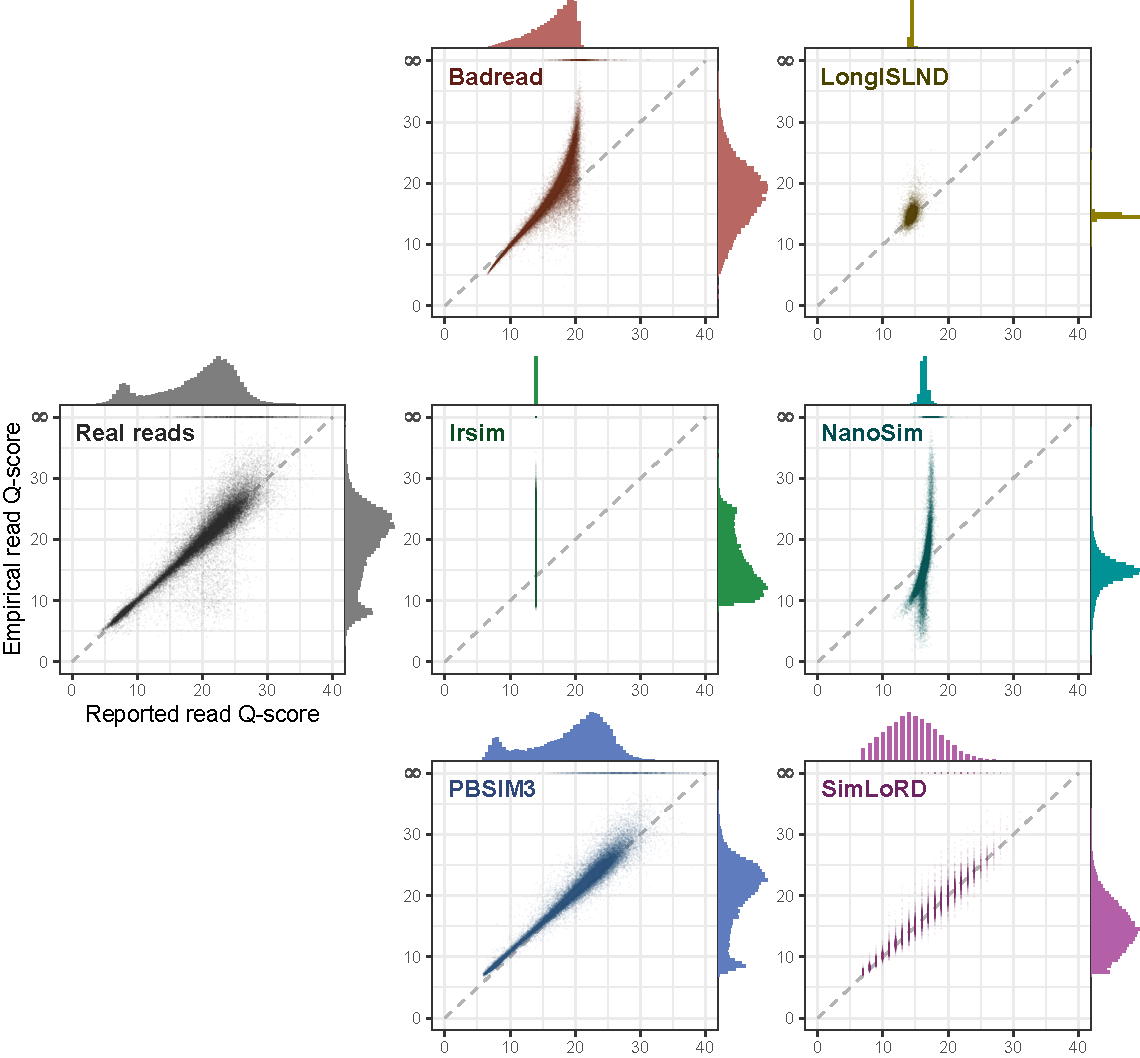
\includegraphics[width=1.0\textwidth]{figure_1.pdf}
\caption[Empirical and reported read Q-scores]{\textbf{Empirical and reported read Q-scores.} In each panel, the central scatter plot shows each aligned read's reported Q-score (x-axis) and empirical Q-score (y-axis). The reported read Q-score was calculated from the FASTQ quality string by converting base Q-scores to error probabilities, averaging those probabilities across the read, and converting the mean error probability back to a Q-score. Only the aligned region of the read was used to calculate reported read Q-score. The empirical read Q-score was calculated from the read-to-reference alignment identity, converted to Q-score. The top y-axis tick is labelled $\infty$ because some reads contained no errors, giving an empirical error rate of zero and therefore an infinite empirical Q-score. The top marginal histogram for each panel shows the distribution of reported read Q-scores, and the right marginal histogram shows the distribution of empirical read Q-scores. Histogram bars are weighted by aligned read length, so the marginal axes represent the number of aligned read bases in each bin. A simulator is more realistic if its plot closely matches that of the real reads. Wasserstein distances to quantify the difference in distributions are available in Table \ref{tab:supp_distance_metrics}.}
\label{fig:read_qscores}
\end{figure*}

Each read that could be aligned to the reference genome was assigned an empirical Q-score, indicating its true accuracy. Each read also had a reported Q-score calculated from its FASTQ quality values. Comparing the joint and marginal distributions of these two Q-scores therefore provided a direct visual measure of how closely each simulated dataset resembled the real reads. Summary statistics of the read accuracy distributions and alignments are in Table \ref{tab:supp_read_accuracy}, and metrics after removing reads with a reported Q-score of <10 are in Table \ref{tab:supp_read_accuracy_q10}.

Only PBSIM3 was able to closely reproduce the signature of the real reads, including their distinctive bimodal distribution with a lower peak at $\sim$Q8 and a higher peak at $\sim$Q23 (Figure \ref{fig:read_qscores}). This likely reflects PBSIM3's sampling-based strategy: it copies read lengths and per-base FASTQ quality strings from training reads, samples template sequences of matching length from the reference genome, and introduces errors according to the sampled Q-scores. PBSIM3's reads only departed from the real reads in a few subtle ways: the real read distributions extended to lower qualities than the PBSIM3 reads, and the real reads had more outliers where empirical and reported Q-scores were in stark disagreement (e.g. reported Q20 but empirical Q10).

All other tools departed from the real-read Q-score distributions. Badread had a wide spread of empirical Q-scores, but its reported Q-scores rarely exceeded Q20. LongISLND produced very narrow distributions, with most reads in the Q14--15 range. lrsim produced a range of empirical Q-scores but did not model reported Q-scores at all, using the same Phred score character for every base in every read. NanoSim produced narrow distributions for both empirical and reported Q-scores. SimLoRD produced wide distributions, but it used only a single Phred score character in each read, leading to a discrete reported Q-score distribution.

When Q-scores were analysed at the per-base level rather than the whole-read level, PBSIM3 was again the most realistic simulator. Badread, LongISLND and PBSIM3 all broadly reproduced the distribution of reported base Q-scores for correctly called bases (Figure \ref{fig:supp_qscore_correct_bases}), but only PBSIM3 also closely matched the distribution of reported base Q-scores for error-associated bases (Figure \ref{fig:supp_qscore_incorrect_bases}) and for the Q-score calibration curve (Figure \ref{fig:supp_qscore_calibration}).


\subsection{Error profiles}

Errors in the real reads were strongly context dependent: the 192 3-mer substitution error rates spanned nearly three orders of magnitude, from 0.0059\% to 3.6\% (Figure \ref{fig:3mer_subs}). This is consistent with ONT sequencing's raw-current signal (the ``squiggle''), in which some \textit{k}-mers produce less distinct signals and are therefore more prone to basecalling errors\cite{krishnakumar2018systematic}. Badread and LongISLND were the only simulators to reproduce this broad pattern, although both produced elevated error rates for substitution types that were rare in the real reads. In contrast, lrsim, NanoSim, PBSIM3 and SimLoRD assigned roughly uniform error rates to all 3-mer substitution types, failing to reproduce the context-specific substitution errors seen in the real reads.

\begin{figure*}[t]
\centering
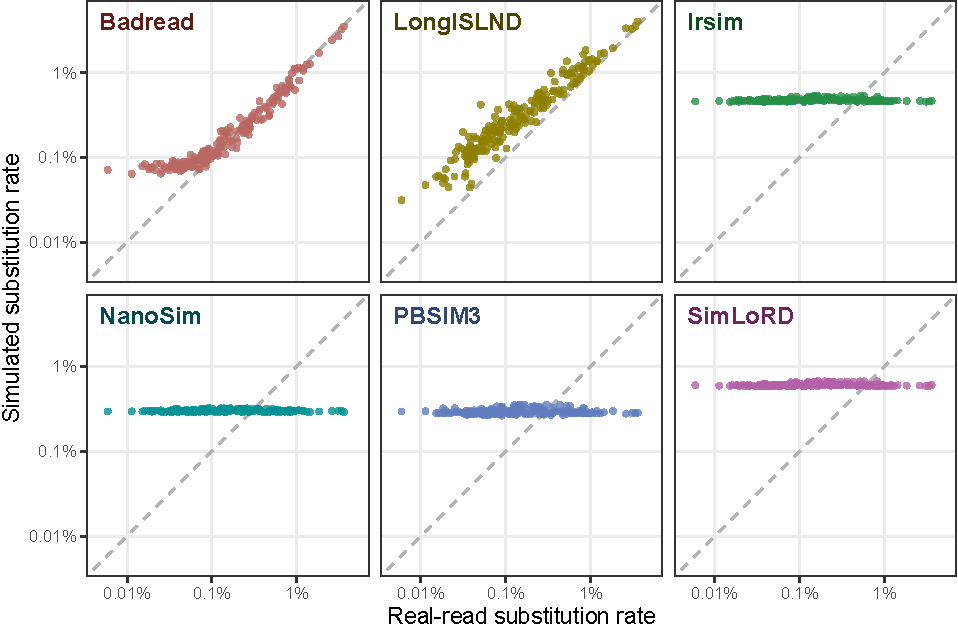
\includegraphics[width=0.84\textwidth]{figure_2.pdf}
\caption[Substitution rates by 3-mer context]{\textbf{Substitution rates by 3-mer context.} Simulated vs real error rates for the 192 distinct 3-mer substitution types, in which only the middle base changes. Each point represents one 3-mer substitution. Real-read error rates range from 0.0059\% (\texttt{CTG}→\texttt{CGG}) to 3.6\% (\texttt{CGA}→\texttt{CAA}). A simulator is more realistic if the points lie close to the diagonal dashed line of equality. Mean absolute error distances to quantify the difference in distributions are available in Table \ref{tab:supp_distance_metrics}.}
\label{fig:3mer_subs}
\end{figure*}

Homopolymer error rates in the real ONT reads rose at an increasing rate as homopolymers became longer (Figure \ref{fig:homopolymer_errors}). LongISLND reproduced this overall pattern most closely, although its curve showed an abrupt drop in error rate from 4-mer to 5-mer homopolymers due to a switch from per-base to whole-homopolymer sampling at length 5. All other tools reproduced this curvature poorly, with error rates that increased linearly with homopolymer length.


\begin{figure}[t]
\centering
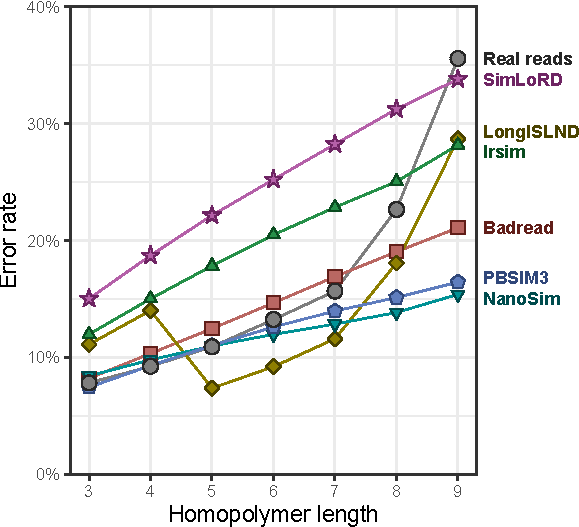
\includegraphics[width=\columnwidth]{figure_3.pdf}
\caption[Homopolymer error rates]{\textbf{Homopolymer error rates.} Homopolymer error rate as reported by Pomoxis, plotted as a function of homopolymer length for real reads and six ONT read simulators. Error rate is defined here as the fraction of reads in which the homopolymer length was not represented correctly. Observation counts and numbers of distinct reference loci are in Table \ref{tab:supp_homopolymer_counts}. Homopolymers of length 10 were excluded from this plot due to there being only two instances in the reference genome. A simulator is more realistic if its curve closely matches that of the real reads. Mean absolute error distances to quantify the difference in distributions are available in Table \ref{tab:supp_distance_metrics}.}
\label{fig:homopolymer_errors}
\end{figure}


\subsection{Assembly accuracy}

Assembly accuracy vs read depth plots are in Figure \ref{fig:supp_assemblies}. For the real reads, assembly accuracy improved with depth, up to $\sim$30$\times$ depth. Assemblies of real reads only achieved perfect accuracy (zero errors) three times. Assemblies of LongISLND simulated reads best matched this pattern, however Raven assemblies of LongISLND reads had notably lower accuracy. Badread, lrsim, PBSIM3 and SimLoRD all produced assemblies that were too accurate (frequently with no detected errors), indicating poor or incomplete modelling of systematic errors in ONT reads. NanoSim simulated reads had strong assembler-specific effects, with Flye assemblies often having zero errors but metaMDBG assemblies were very low accuracy.


\subsection{Computational resources}

Computational time and memory usage for each tool are listed in Table \ref{tab:supp_resources}. Badread was the slowest tool tested, taking over 9 hours to complete its training step and over 30 minutes to complete its simulation step. When considering all steps, PBSIM3 was the overall fastest tool, taking $\sim$1.5 minutes to complete. When considering only the simulation step, lrsim was the fastest, completing in $\sim$1 second. NanoSim used the most memory, peaking at over 59 GB during its training step. PBSIM3 was the most memory efficient, using only $\sim$20 MB.



\section{Discussion}

This study benchmarked six ONT‑compatible read simulators against contemporary R10.4.1 ONT real reads, with the goal of identifying which tools best reproduce empirical read characteristics. That is, we judged simulators by how closely their outputs matched real reads across features relevant to downstream use, such as method development and pipeline validation. Our results demonstrate that no simulator perfectly captures all aspects of modern ONT reads, but PBSIM3, Badread and LongISLND performed best, depending on the key metric considered.

PBSIM3 performed strongly overall and was the most realistic simulator for several key properties of the read sets. Its simulated reads closely matched the real data in read length, empirical read accuracy and FASTQ Q-scores (Figure \ref{fig:read_qscores}), making it a practical choice for users who want simulated datasets that resemble real ONT whole-genome sequencing output in broad terms. This realism likely comes from its sampling-based approach, where quality strings are copied from empirical data rather than generated de novo. However, a limitation of PBSIM3 was that it was less successful at reproducing the error profile of the real data (Figures \ref{fig:3mer_subs} and \ref{fig:homopolymer_errors}).

Badread offers users parametric control over the simulated reads, which can be valuable when specific read-set properties are needed. This flexibility came at the expense of realism: its read length and accuracy distributions deviated from those of the real reads (Figures \ref{fig:supp_read_length} and \ref{fig:read_qscores}). Badread modelled substitution errors well (Figure \ref{fig:3mer_subs}) but captured homopolymer-length errors less well (Figure \ref{fig:homopolymer_errors}). Further, as Badread is implemented entirely in Python, it was slower to run than other tools.

LongISLND performed well at modelling substitutions (Figure \ref{fig:3mer_subs}), error rates in longer homopolymers (\ref{fig:homopolymer_errors}) and reproducing assembly errors (Figure \ref{fig:supp_assemblies}). However, its distributions of empirical and reported read Q-scores were unrealistically narrow, limiting its potential use as a simulator (Figure \ref{fig:read_qscores}).

The remaining simulators were less suitable for realistic ONT read simulation. lrsim and SimLoRD were limited by their treatment of FASTQ Q-scores: lrsim assigns the same Q-score to every base in the entire output, while SimLoRD assigns a single Q-score per read. This makes both tools unsuitable for applications which use per-base Q-scores. NanoSim produced an unrealistically narrow distribution of read-level accuracy (Figure \ref{fig:read_qscores}) and an unrealistically broad distribution of base-level accuracy (Figures \ref{fig:supp_qscore_correct_bases} and \ref{fig:supp_qscore_incorrect_bases}).

In this study, we did not exhaustively explore every possible configuration of each tool. We aimed to run each one in the way that we judged most likely to maximise overall realism. Other configurations may have produced different results. For example, PBSIM3 includes an error-model HMM mode that may improve error realism, but this comes with trade-offs: read lengths and Q-scores are then generated from parametric models rather than sampled from empirical data, and it does not support training a custom model on user-provided data.

Another limitation is that our benchmarking focused only on WGS. Other applications of long-read sequencing, such as transcriptomics, amplicons and metagenomics, may prioritise different properties of simulated reads. We also did not assess how reads were distributed across the reference genome. Real sequencing datasets may show positional biases in read start sites or coverage, arising from library preparation, sequence composition or other experimental factors, and these biases could be important for some downstream analyses.

This study used a single \textit{Listeria innocua} genome, sequenced using an R10.4.1 ONT flow cell and basecalled with Dorado's \texttt{sup@v5.2.0} model. This dataset was a practical choice because its highly accurate reference genome allowed for detailed analyses, and its small genome size limited computational requirements. Our findings are limited to the dataset and simulator configurations tested. Although the metrics we assessed are not specific to bacterial genomics, it remains to be evaluated whether the conclusions of this study generalise more broadly. Future work could test these simulators on other organisms (e.g. humans), sequencing chemistries, basecalling models and platforms (e.g. PacBio HiFi).



\section{Conclusions}

In the setting of ONT bacterial WGS, no simulator produced reads that looked realistic across all tested metrics. When used in its sampling-based mode, PBSIM3 is likely the best choice for many users. It was easy to run, fast to execute and performed well on several key properties of ONT whole-genome sequencing data, particularly read length and read-level accuracy metrics, although it failed to model error types well. Badread did better at modelling some error types and offers parametric control over the simulated read set, but at the cost of less realism and substantially slower run times. LongISLND modelled some error types well, but its simulated reads had an unrealistically narrow accuracy distribution. The remaining simulators each showed limitations that make them less suitable for general use. More broadly, the fact that no tool performed well on all metrics highlights an opportunity for improved long-read simulators that can combine realistic read-level distributions with more faithful modelling of sequencing errors.




\section{Availability of data and materials}

Detailed commands, custom scripts and complete analysis outputs are publicly available at: \href{https://github.com/mtaouk/ONT-Read-Simulator-Benchmarking}{\nolinkurl{github.com/mtaouk/ONT-Read-Simulator-Benchmarking}}.

The reference genome and full read sets used in this study are available at: \href{https://doi.org/10.26188/32194977}{\nolinkurl{doi.org/10.26188/32194977}}.



\section{Competing interests}

The authors declare that there are no conflicts of interest.




\section{Funding}

This work was supported by the Australian Research Council Discovery Early Career Researcher Award [DE250100677 to R.R.W.], Emerging Leadership Fellowship from the National Health and Medical Research Council of Australia [2041653 to D.J.I.] and the Research Accelerator Fund -- Bioinformatics 2024 generously supported by Doherty Institute philanthropic donations [to D.J.I.].




\section{Authors' contributions}

R.R.W. conceived the study. M.L.T. and R.R.W. performed analyses and drafted the manuscript. D.J.I. and R.R.W. supervised the work, contributed to study design and interpretation of results, and revised the manuscript critically. All authors read and approved the final manuscript.



\bibliographystyle{custom_unsrt}
\bibliography{references}



\clearpage
\onecolumn
\renewcommand{\thetable}{S\arabic{table}}
\renewcommand{\thefigure}{S\arabic{figure}}
\setcounter{table}{0}
\setcounter{figure}{0}



\section*{Supplementary Information}

\noindent Supplementary methods are available at: \href{https://github.com/mtaouk/ONT-Read-Simulator-Benchmarking}{\nolinkurl{github.com/mtaouk/ONT-Read-Simulator-Benchmarking}}.


\par\vspace{2.0em}


\begin{table}[!htbp]
\centering
\scriptsize
\caption[Read length statistics]{\textbf{Read length statistics.}}
\label{tab:supp_read_stats}
\renewcommand{\arraystretch}{1.15}
\begin{tabular}{
>{\raggedright\arraybackslash}m{0.08\textwidth}
>{\raggedleft\arraybackslash}m{0.08\textwidth}
>{\raggedleft\arraybackslash}m{0.10\textwidth}
>{\raggedleft\arraybackslash}m{0.07\textwidth}
>{\raggedleft\arraybackslash}m{0.08\textwidth}
>{\raggedleft\arraybackslash}m{0.08\textwidth}
>{\raggedleft\arraybackslash}m{0.08\textwidth}
}
\toprule
\textbf{Dataset} &
\textbf{Number of reads} &
\textbf{Total bases (bp)} &
\textbf{Min length (bp)} &
\textbf{Max length (bp)} &
\textbf{Mean length (bp)} &
\textbf{N50 length (bp)} \\
\midrule
Real reads & 53,093 & 297,265,978 &  5 & 826,029 & 5,599.0 &  8,994 \\
\midrule
Badread    & 53,180 & 297,256,127 &  1 &  78,973 & 5,589.6 & 10,558 \\
\midrule
LongISLND  & 53,956 & 297,851,844 & 37 & 181,950 & 5,520.3 &  8,758 \\
\midrule
lrsim      & 53,013 & 297,445,673 & 10 &  89,609 & 5,610.8 &  8,869 \\
\midrule
NanoSim    & 53,227 & 309,873,325 & 50 & 214,233 & 5,821.7 &  8,771 \\
\midrule
PBSIM3     & 53,503 & 297,258,351 & 93 & 107,108 & 5,555.9 &  8,784 \\
\midrule
SimLoRD    & 53,202 & 300,580,690 &  5 & 700,862 & 5,649.8 &  9,033 \\
\bottomrule
\end{tabular}
\end{table}


\begin{table}[!htbp]
\centering
\scriptsize
\caption[Read accuracy and alignment statistics]{\textbf{Read accuracy and alignment statistics.} For empirical and reported Q-scores, the mean and standard deviation (SD) values are weighted by aligned read length. Reads without any errors in their alignments have an empirical Q-score of Q$\infty$ and were therefore excluded from the empirical Q-score mean and SD calculations. The ``Unaligned reads'' column shows the percentage of reads without any alignment to the reference genome. The ``Unaligned bases'' column shows the percentage of total read bases which were not part of each read's best alignment, e.g. from unaligned regions at the start or end of reads. Error types are expressed as percentages of all aligned erroneous bases, with insertions and deletions counted by length.}
\label{tab:supp_read_accuracy}
\renewcommand{\arraystretch}{1.15}
\begin{tabular}{
>{\raggedright\arraybackslash}m{0.08\textwidth}
*{4}{>{\raggedleft\arraybackslash}m{0.05\textwidth}}
*{3}{>{\raggedleft\arraybackslash}m{0.06\textwidth}}
*{2}{>{\raggedleft\arraybackslash}m{0.08\textwidth}}
}
\toprule
& \multicolumn{2}{c}{\makecell{\textbf{Empirical}\\\textbf{Q-score}}} & \multicolumn{2}{c}{\makecell{\textbf{Reported}\\\textbf{Q-score}}} & \multicolumn{3}{c}{\textbf{Error types}} & & \\
\cmidrule(lr){2-3}\cmidrule(lr){4-5}\cmidrule(lr){6-8}
\textbf{Dataset} & \textbf{Mean} & \textbf{SD} & \textbf{Mean} & \textbf{SD} & \makecell[r]{\textbf{Substi-}\\\textbf{tutions}} & \makecell[r]{\textbf{Inser-}\\\textbf{tions}} & \makecell[r]{\textbf{Dele-}\\\textbf{tions}} & \textbf{Unaligned reads} & \textbf{Unaligned bases} \\
\midrule
Real reads & 18.98 & 6.07 & 19.24 & 5.84 & 40.1\% & 18.9\% & 41.0\% & 1.06\% & 1.88\% \\
\midrule
Badread & 18.20 & 5.06 & 16.48 & 3.16 & 39.8\% & 17.9\% & 42.4\% & 6.44\% & 4.06\% \\
\midrule
LongISLND & 14.69 & 0.34 & 14.39 & 0.18 & 42.1\% & 16.8\% & 41.1\% & 0.24\% & 0.01\% \\
\midrule
lrsim & 16.06 & 4.64 & 14.00 & 0.00 & 43.8\% & 21.7\% & 34.4\% & 0.18\% & 0.02\% \\
\midrule
NanoSim & 14.89 & 3.01 & 16.29 & 0.46 & 32.3\% & 12.7\% & 54.9\% & 1.14\% & 2.50\% \\
\midrule
PBSIM3 & 19.89 & 5.68 & 19.30 & 5.78 & 46.8\% & 13.8\% & 39.4\% & 0.19\% & 0.17\% \\
\midrule
SimLoRD & 14.77 & 3.97 & 14.64 & 4.03 & 44.4\% & 17.9\% & 37.7\% & 0.90\% & 0.05\% \\
\bottomrule
\end{tabular}
\end{table}

\begin{table}[!htbp]
\centering
\scriptsize
\caption[Read accuracy and alignment statistics after Q10 filtering]{\textbf{Read accuracy and alignment statistics after Q10 filtering.} This table contains the same data as Table \ref{tab:supp_read_accuracy}, but after reads with a reported Q-score of <10 are removed.}
\label{tab:supp_read_accuracy_q10}
\renewcommand{\arraystretch}{1.15}
\begin{tabular}{
>{\raggedright\arraybackslash}m{0.08\textwidth}
*{4}{>{\raggedleft\arraybackslash}m{0.05\textwidth}}
*{3}{>{\raggedleft\arraybackslash}m{0.06\textwidth}}
*{2}{>{\raggedleft\arraybackslash}m{0.08\textwidth}}
}
\toprule
& \multicolumn{2}{c}{\makecell{\textbf{Empirical}\\\textbf{Q-score}}} & \multicolumn{2}{c}{\makecell{\textbf{Reported}\\\textbf{Q-score}}} & \multicolumn{3}{c}{\textbf{Error types}} & & \\
\cmidrule(lr){2-3}\cmidrule(lr){4-5}\cmidrule(lr){6-8}
\textbf{Dataset} & \textbf{Mean} & \textbf{SD} & \textbf{Mean} & \textbf{SD} & \makecell[r]{\textbf{Substi-}\\\textbf{tutions}} & \makecell[r]{\textbf{Inser-}\\\textbf{tions}} & \makecell[r]{\textbf{Dele-}\\\textbf{tions}} & \textbf{Unaligned reads} & \textbf{Unaligned bases} \\
\midrule
Real reads & 20.53 & 4.76 & 20.84 & 4.26 & 35.1\% & 18.2\% & 46.8\% & 0.40\% & 0.71\% \\
\midrule
Badread & 18.71 & 4.63 & 16.86 & 2.71 & 38.0\% & 19.3\% & 42.7\% & 4.43\% & 2.87\% \\
\midrule
LongISLND & 14.69 & 0.34 & 14.39 & 0.18 & 42.1\% & 16.8\% & 41.1\% & 0.24\% & 0.01\% \\
\midrule
lrsim & 16.06 & 4.64 & 14.00 & 0.00 & 43.8\% & 21.7\% & 34.4\% & 0.18\% & 0.02\% \\
\midrule
NanoSim & 14.88 & 3.00 & 16.29 & 0.45 & 32.3\% & 12.8\% & 54.9\% & 0.09\% & 0.66\% \\
\midrule
PBSIM3 & 21.33 & 4.32 & 20.78 & 4.35 & 46.1\% & 14.3\% & 39.6\% & 0.00\% & 0.08\% \\
\midrule
SimLoRD & 15.53 & 3.53 & 15.43 & 3.54 & 43.1\% & 17.8\% & 39.1\% & 0.50\% & 0.02\% \\
\bottomrule
\end{tabular}
\end{table}

\begin{table}[!htbp]
\centering
\scriptsize
\caption[Distances between simulated-read and real-read distributions]{\textbf{Distances between simulated-read and real-read distributions.} Distance metrics comparing the simulated reads to the real reads for the following distributions: read length (Figure \ref{fig:supp_read_length}), empirical read Q-score (Figure \ref{fig:read_qscores} y-axis), reported read Q-score (Figure \ref{fig:read_qscores} x-axis), correct base Q-score (Figure \ref{fig:supp_qscore_correct_bases}), error base Q-score (Figure \ref{fig:supp_qscore_incorrect_bases}), 3-mer substitutions (Figure \ref{fig:3mer_subs}) and homopolymer length errors (Figure \ref{fig:homopolymer_errors}).
\par\smallskip
For the read length and Q-score distributions, the values are Wasserstein-1 distances. Read lengths are weighted by full read length, and read Q-scores are weighted by aligned read length. Reported read Q-scores are calculated over the aligned interval, and reads without any errors in their alignments have an empirical Q-score of Q$\infty$ and were therefore excluded from the empirical Q-score distance.
\par\smallskip
For the 3-mer substitutions and homopolymer-length errors, the values are mean absolute errors (MAE). For the 3-mer substitutions, these were calculated in log$_{10}$ space to match the plots in Figure \ref{fig:3mer_subs}. For the homopolymer-length errors, 10-mers were excluded due to their low frequency (Table \ref{tab:supp_homopolymer_counts}).
\par\smallskip
Units for the distances are as follows. Read-length distances are expressed in bp, Q-score distances in Phred-score units, 3-mer substitution MAEs in log$_{10}$ units, and homopolymer-error MAEs in percentage points. Smaller values indicate a closer match between the simulated-read and real-read distributions, and a value of zero would indicate perfect agreement.
}
\label{tab:supp_distance_metrics}
\renewcommand{\arraystretch}{1.15}
\begin{tabular}{
>{\raggedright\arraybackslash}m{0.10\textwidth}
*{7}{>{\raggedleft\arraybackslash}m{0.08\textwidth}}
}
\toprule
\textbf{Simulator} &
\makecell[r]{\textbf{Read}\\\textbf{length}} &
\makecell[r]{\textbf{Empirical}\\\textbf{read}\\\textbf{Q-score}} &
\makecell[r]{\textbf{Reported}\\\textbf{read}\\\textbf{Q-score}} &
\makecell[r]{\textbf{Correct}\\\textbf{base}\\\textbf{Q-score}} &
\makecell[r]{\textbf{Error}\\\textbf{base}\\\textbf{Q-score}} &
\makecell[r]{\textbf{3-mer}\\\textbf{substi-}\\\textbf{tutions}} &
\makecell[r]{\textbf{Homo-}\\\textbf{polymer}\\\textbf{errors}} \\
\midrule
Badread & 3382 & 1.54 & 3.47 & 0.69 & 4.57 & 0.161 & 3.40 \\
\midrule
LongISLND & 2265 & 6.34 & 6.68 & 0.71 & 7.62 & 0.332 & 4.46 \\
\midrule
lrsim & 2413 & 3.55 & 7.01 & 23.98 & 7.70 & 0.652 & 5.87 \\
\midrule
NanoSim & 2484 & 4.83 & 5.49 & 9.16 & 8.07 & 0.547 & 4.90 \\
\midrule
PBSIM3 & 2430 & 0.92 & 0.07 & 0.10 & 0.51 & 0.541 & 4.22 \\
\midrule
SimLoRD & 2570 & 4.43 & 4.74 & 22.02 & 4.60 & 0.720 & 8.98 \\
\bottomrule
\end{tabular}
\end{table}



\begin{table}[!htbp]
\centering
\scriptsize
\setlength{\tabcolsep}{3pt}
\caption[Homopolymer observation counts]{\textbf{Homopolymer counts.}}
\label{tab:supp_homopolymer_counts}
\renewcommand{\arraystretch}{1.15}
\begin{tabular}{
>{\raggedright\arraybackslash}m{0.11\textwidth}
>{\raggedleft\arraybackslash}m{0.08\textwidth}
*{7}{>{\raggedleft\arraybackslash}m{0.098\textwidth}}
}
\toprule
\textbf{Homopolymer length (bp)} &
\textbf{Reference genome} &
\textbf{Real reads} &
\textbf{Badread} &
\textbf{LongISLND} &
\textbf{lrsim} &
\textbf{NanoSim} &
\textbf{PBSIM3} &
\textbf{SimLoRD} \\
\midrule
3 & 119,016 & 11,729,323 & 11,494,777 & 12,017,356 & 11,957,966 & 12,307,437 & 11,964,750 & 12,138,826 \\
\midrule
4 & 46,166 & 4,543,083 & 4,456,504 & 4,652,688 & 4,631,860 & 4,767,371 & 4,634,121 & 4,707,153 \\
\midrule
5 & 18,220 & 1,780,934 & 1,761,228 & 1,837,558 & 1,829,352 & 1,882,221 & 1,828,026 & 1,852,669 \\
\midrule
6 & 6,826 & 664,649 & 657,329 & 688,895 & 684,970 & 705,043 & 684,622 & 696,158 \\
\midrule
7 & 2,607 & 249,186 & 250,785 & 262,156 & 260,439 & 267,959 & 261,605 & 265,312 \\
\midrule
8 & 269 & 23,891 & 25,920 & 26,490 & 26,778 & 27,114 & 26,821 & 27,244 \\
\midrule
9 & 22 & 1,762 & 1,929 & 1,867 & 2,157 & 1,922 & 1,848 & 1,937 \\
\midrule
10 & 2 & 139 & 173 & 115 & 192 & 112 & 143 & 126 \\
\bottomrule
\end{tabular}
\end{table}


\begin{table}[!htbp]
\centering
\scriptsize
\caption[Computational resources]{\textbf{Computational resources.} Wall-clock execution time and maximum RAM usage for training and simulation commands. PBSIM3 and SimLoRD do not have a separate training step and so only list simulation times. All tools were run on a server with Dual AMD EPYC 7742 CPUs, 128 cores (256 threads) 503 GB RAM, running Red Hat Enterprise Linux 10.2.
\par\smallskip
Commands were run with 16 threads when possible. lrsim (simulation step) and NanoSim support multithreading and were run using 16 threads. Badread, LongISLND, lrsim (training step), PBSIM3 and SimLoRD do not support multithreading and were therefore run with one thread, but all read alignment commands were run with 16 threads.
}
\label{tab:supp_resources}
\renewcommand{\arraystretch}{1.15}
\begin{tabular}{
>{\raggedright\arraybackslash}m{0.10\textwidth}
>{\raggedleft\arraybackslash}m{0.11\textwidth}
>{\raggedleft\arraybackslash}m{0.11\textwidth}
>{\raggedleft\arraybackslash}m{0.11\textwidth}
>{\raggedleft\arraybackslash}m{0.11\textwidth}
}
\toprule
& \multicolumn{2}{c}{\textbf{Training}} & \multicolumn{2}{c}{\textbf{Simulation}} \\
\cmidrule(lr){2-3}\cmidrule(lr){4-5}
\textbf{Tool} &
\textbf{Elapsed time (h:m:s)} &
\textbf{Peak memory (GB)} &
\textbf{Elapsed time (h:m:s)} &
\textbf{Peak memory (GB)} \\
\midrule
Badread   & 9:01:56 & 12.99 & 0:31:30 & 0.42 \\
\midrule
LongISLND & 0:14:57 & 6.39 & 0:04:26 & 14.49 \\
\midrule
lrsim     & 0:03:18 & 6.21 & 0:00:01 & 0.13 \\
\midrule
NanoSim   & 0:38:24 & 59.07 & 0:00:28 & 0.51 \\
\midrule
PBSIM3    & {---} & {---} & 0:01:32 & 0.02 \\
\midrule
SimLoRD   & {---} & {---} & 0:02:47 & 0.19 \\
\bottomrule
\end{tabular}
\end{table}




\begin{figure}[!htbp]
\centering
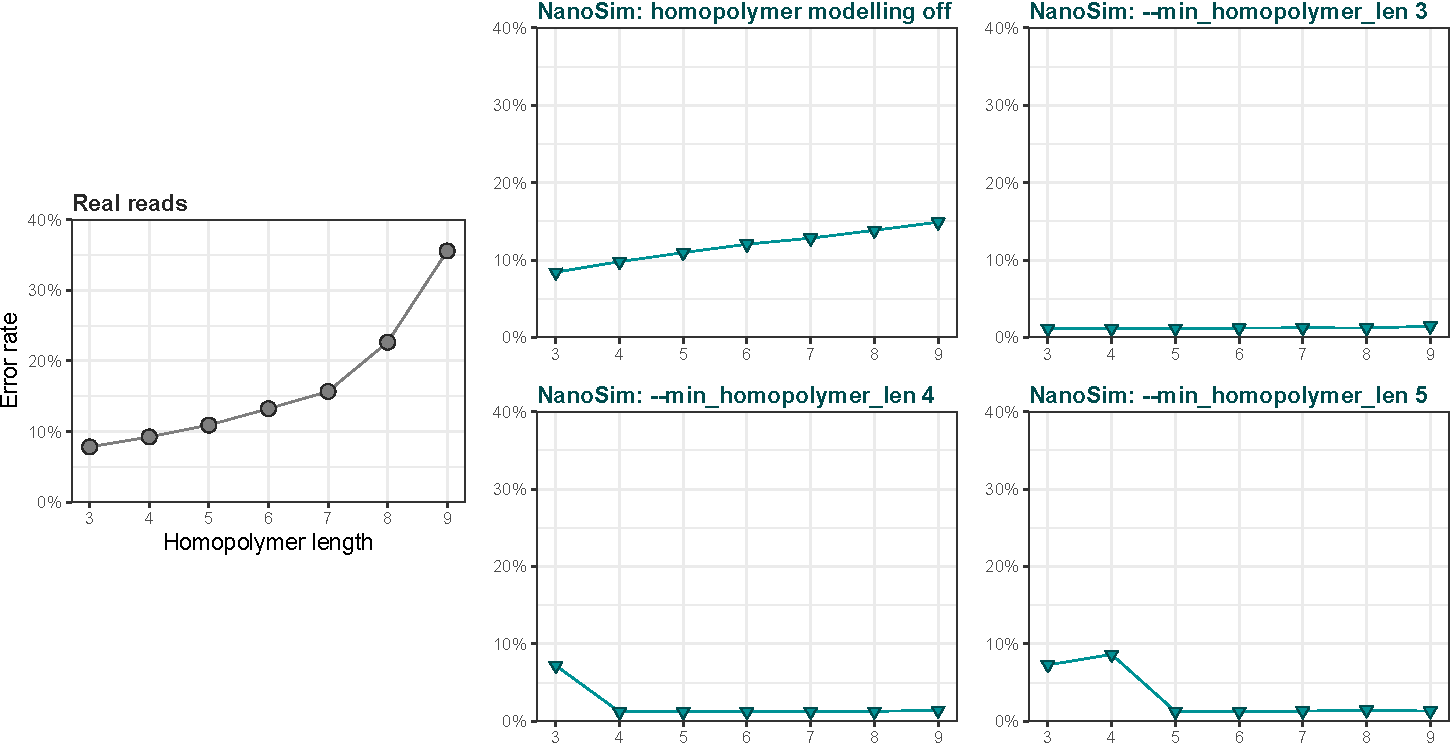
\includegraphics[width=0.8\textwidth]{figure_s1.pdf}
\caption[NanoSim homopolymer modes]{\textbf{NanoSim homopolymer modes.} To test NanoSim's homopolymer-length modelling, we ran NanoSim's read modelling step (\texttt{read\_analysis.py genome}) using \texttt{-hp -{}-min\_homopolymer\_len} \textit{h} and NanoSim read simulation (\texttt{simulator.py genome}) using \texttt{-hp -k} \textit{h}. We tested values of \textit{h} ranging from 3--5 (values of 6 or greater caused NanoSim to crash), as well as no homopolymer modelling.
\par\smallskip
Despite intending to improve the realism of homopolymer-length errors, this modelling produced unrealistically low error rates at homopolymers at and above the value of \textit{h}. This appears to result from a bug in NanoSim's training that biases its homopolymer model towards unrealistically low error rates. For the main results in this manuscript, we therefore did not use NanoSim's homopolymer length modelling.}
\label{fig:supp_nanosim_homopolymers}
\end{figure}




\begin{figure}[!htbp]
\centering
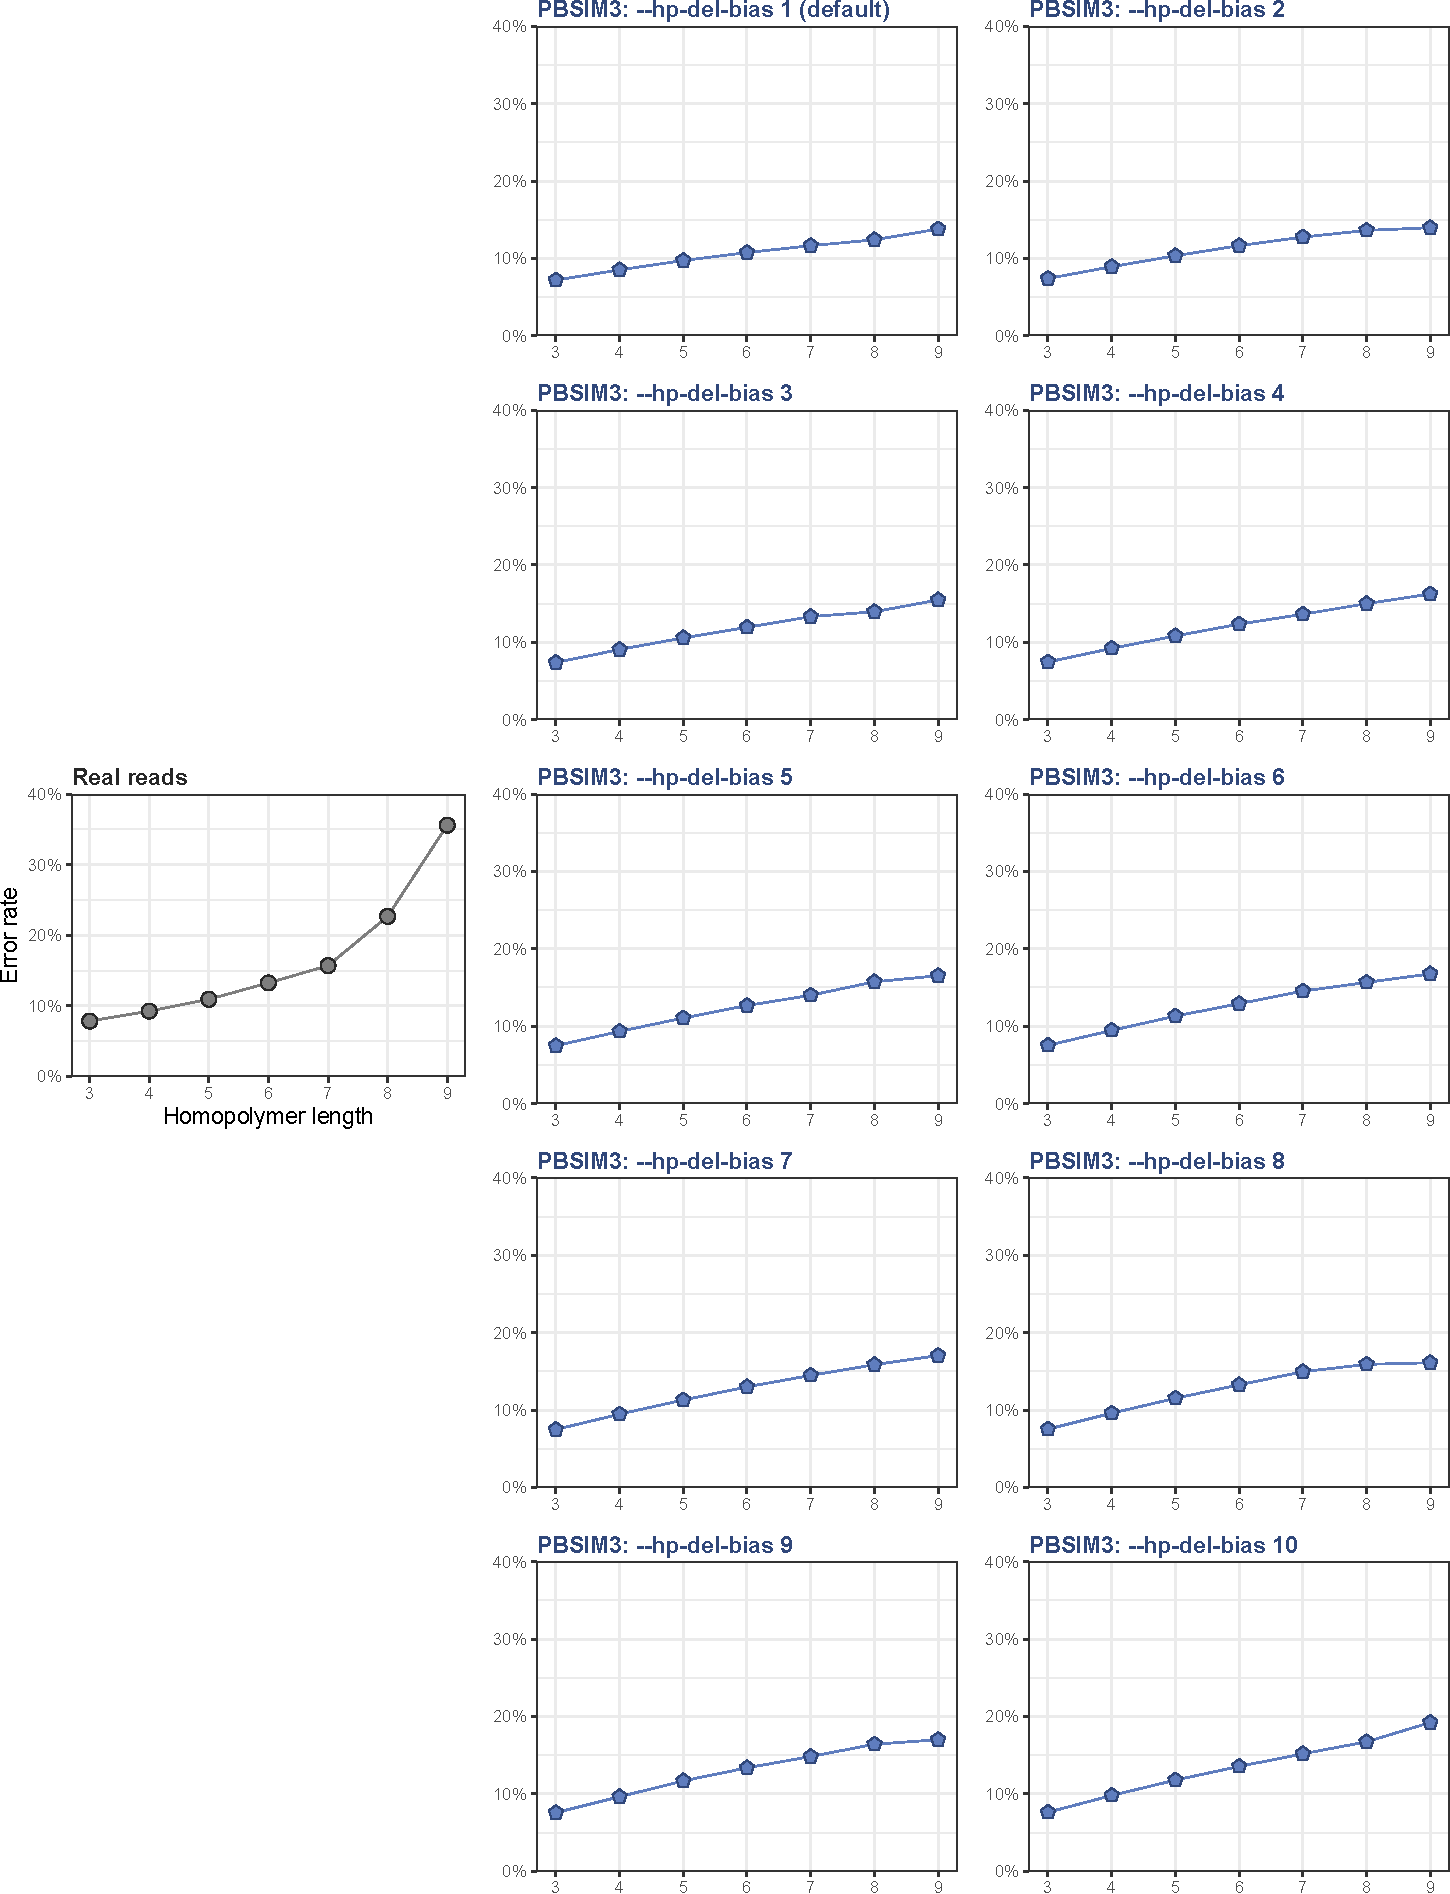
\includegraphics[width=0.8\textwidth]{figure_s2.pdf}
\caption[PBSIM3 homopolymer modes]{\textbf{PBSIM3 homopolymer modes.} PBSIM3 contains a \texttt{-{}-hp-del-bias} option which aims to simulate homopolymer deletion bias in ONT reads. To test this, we ran PBSIM3 using \texttt{-{}-hp-del-bias} \textit{h} using values of \textit{h} ranging from 1--10 (the full range for this option). While higher values of \textit{h} did produce more errors in longer homopolymers, it did not reproduce the inflection of the curve seen with the real reads. For the main results in this manuscript, we used \texttt{-{}-hp-del-bias 5} since that minimised the discrepancy between the real reads' homopolymer errors and PBSIM3's homopolymer errors (weighting the discrepancy using homopolymer occurrences).}
\label{fig:supp_pbsim3_homopolymers}
\end{figure}




\begin{figure}[!htbp]
\centering
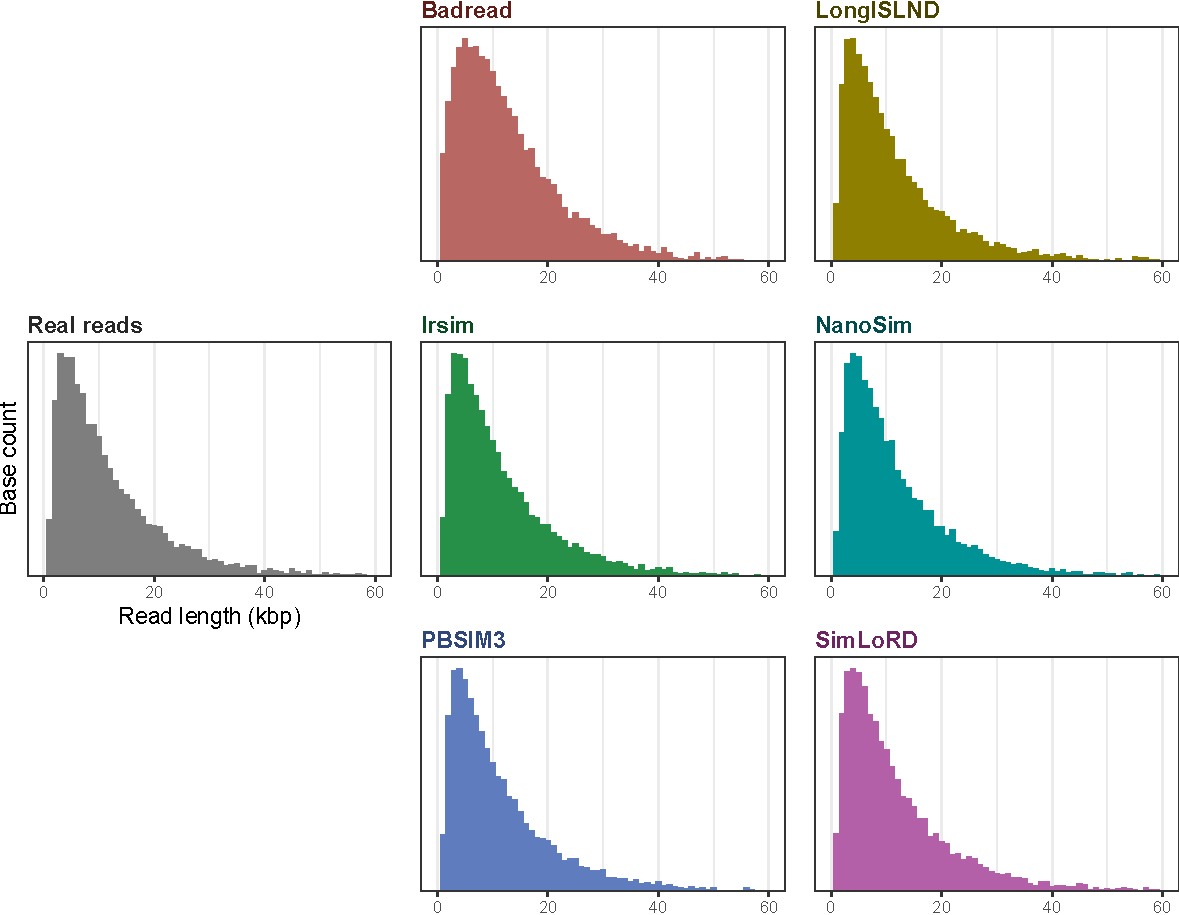
\includegraphics[width=0.69\textwidth]{figure_s3.pdf}
\caption[Read length distributions]{\textbf{Read length distributions.} Histograms are shown for the real and simulated datasets. The x-axis shows read length in 1 kbp bins. Histogram bars are weighted by read length, so the y-axis represents the total number of bases contributed by reads in each length bin rather than the number of reads. A simulator is more realistic if its histogram closely matches that of the real reads. Wasserstein distances to quantify the difference in distributions are available in Table \ref{tab:supp_distance_metrics}.}
\label{fig:supp_read_length}
\end{figure}




\begin{figure}[!htbp]
\centering
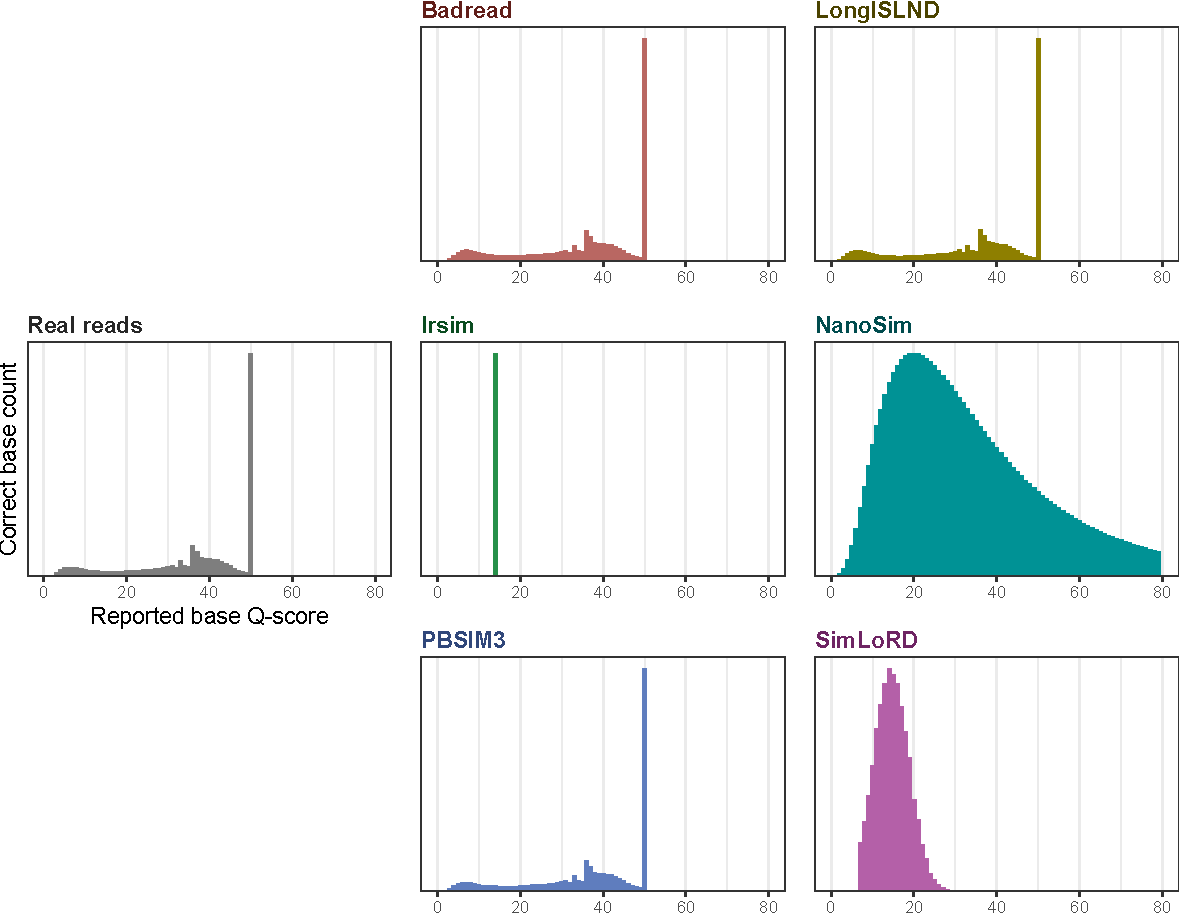
\includegraphics[width=0.69\textwidth]{figure_s4.pdf}
\caption[Correct base Q-score distribution]{\textbf{Correct base Q-score distribution.} Reported base Q-score distributions for correctly called bases in the real and simulated datasets. In each panel, bars show the number of bases in each reported base Q-score bin. A base was counted as correct only if it matched the reference and was not adjacent to a deletion in the alignment. A simulator is more realistic if its histogram closely matches that of the real reads. Wasserstein distances to quantify the difference in distributions are available in Table \ref{tab:supp_distance_metrics}.}
\label{fig:supp_qscore_correct_bases}
\end{figure}




\begin{figure}[!htbp]
\centering
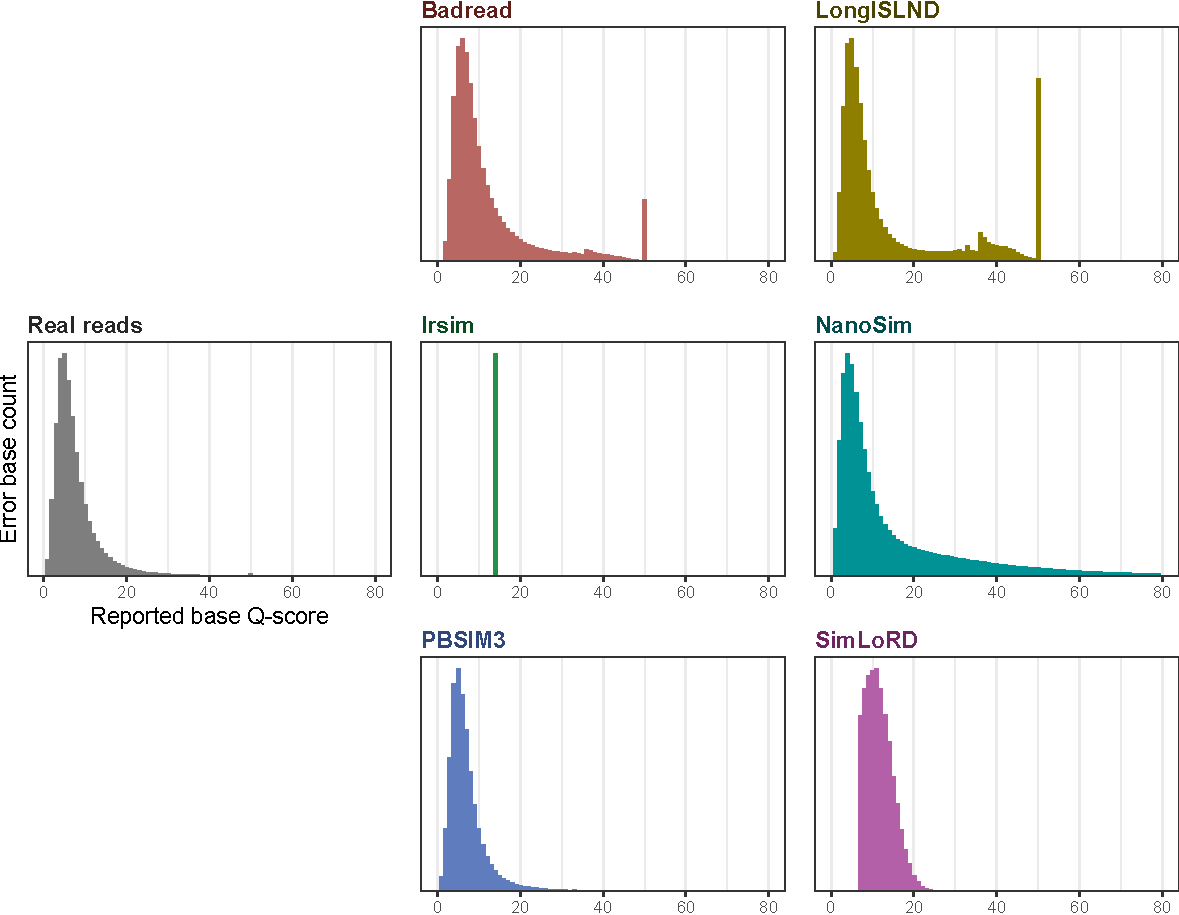
\includegraphics[width=0.69\textwidth]{figure_s5.pdf}
\caption[Error-associated base Q-score distribution]{\textbf{Error-associated base Q-score distribution.} Reported base Q-score distributions for error-associated bases in the real and simulated datasets. In each panel, bars show the number of error-associated bases in each reported base Q-score bin. Error-associated bases were defined as mismatches and insertions, plus deletion-associated events estimated as half the number of matched bases adjacent to deletions, because deleted bases themselves have no reported Q-score. A simulator is more realistic if its histogram closely matches that of the real reads. Wasserstein distances to quantify the difference in distributions are available in Table \ref{tab:supp_distance_metrics}.}
\label{fig:supp_qscore_incorrect_bases}
\end{figure}




\begin{figure}[!htbp]
\centering
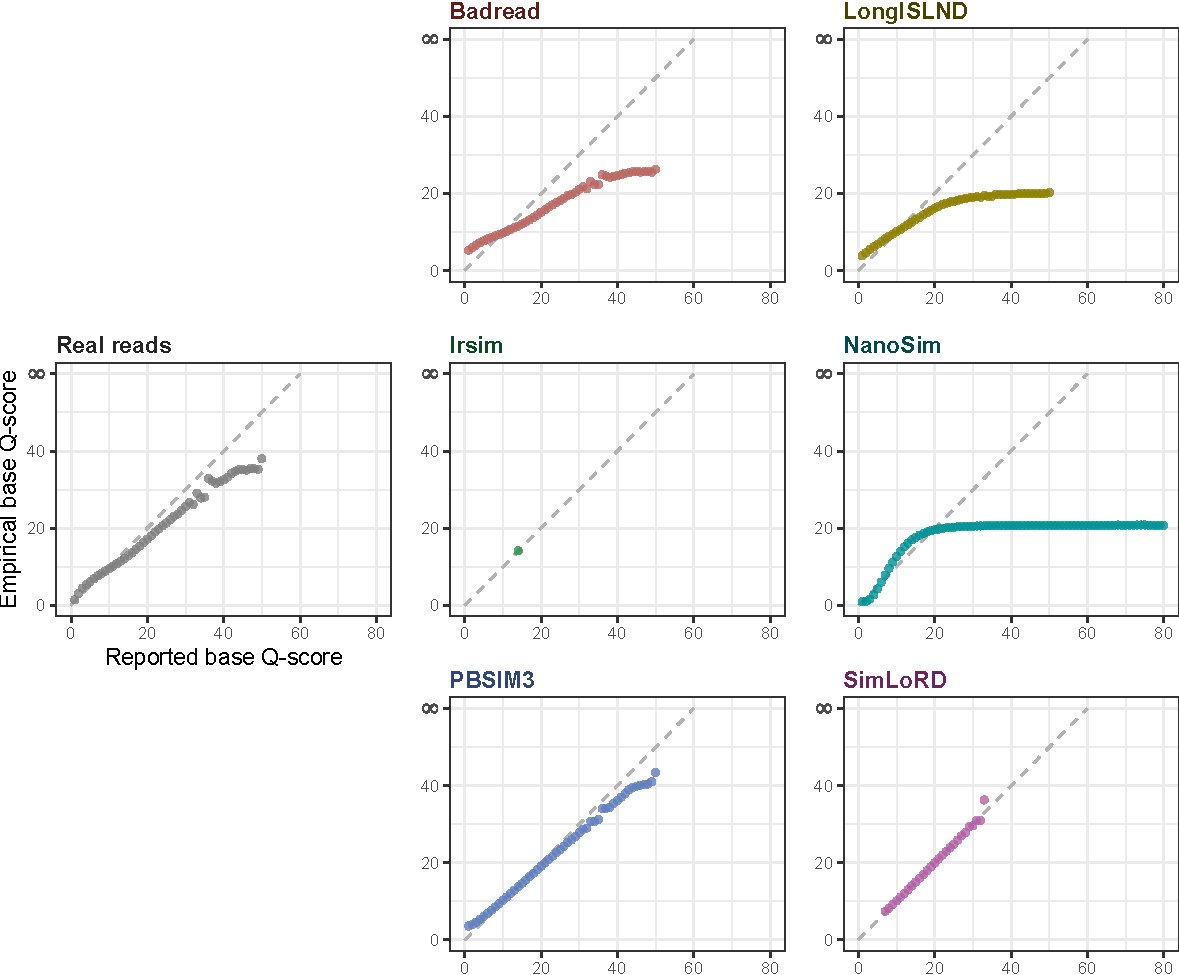
\includegraphics[width=0.69\textwidth]{figure_s6.pdf}
\caption[Q-score calibration curve]{\textbf{Q-score calibration curve.} Per-base Q-score calibration for real and simulated datasets. Each point represents one reported base Q-score bin (x-axis), and its y-value is the empirical base Q-score calculated from the observed error rate among bases with that reported Q-score. For each Q-score bin, the empirical error rate was calculated as $(X + I + D/2)/(M + X + I + D/2)$, where $X$ is the count of mismatching bases, $I$ is the count of inserted bases, $D$ is the count of matching bases adjacent to a deletion (regardless of the number of deleted bases) and $M$ is the count of matching bases not adjacent to a deletion. The dashed diagonal indicates perfect calibration, where reported and empirical base Q-scores are equal.}
\label{fig:supp_qscore_calibration}
\end{figure}





\begin{figure}[!htbp]
\centering
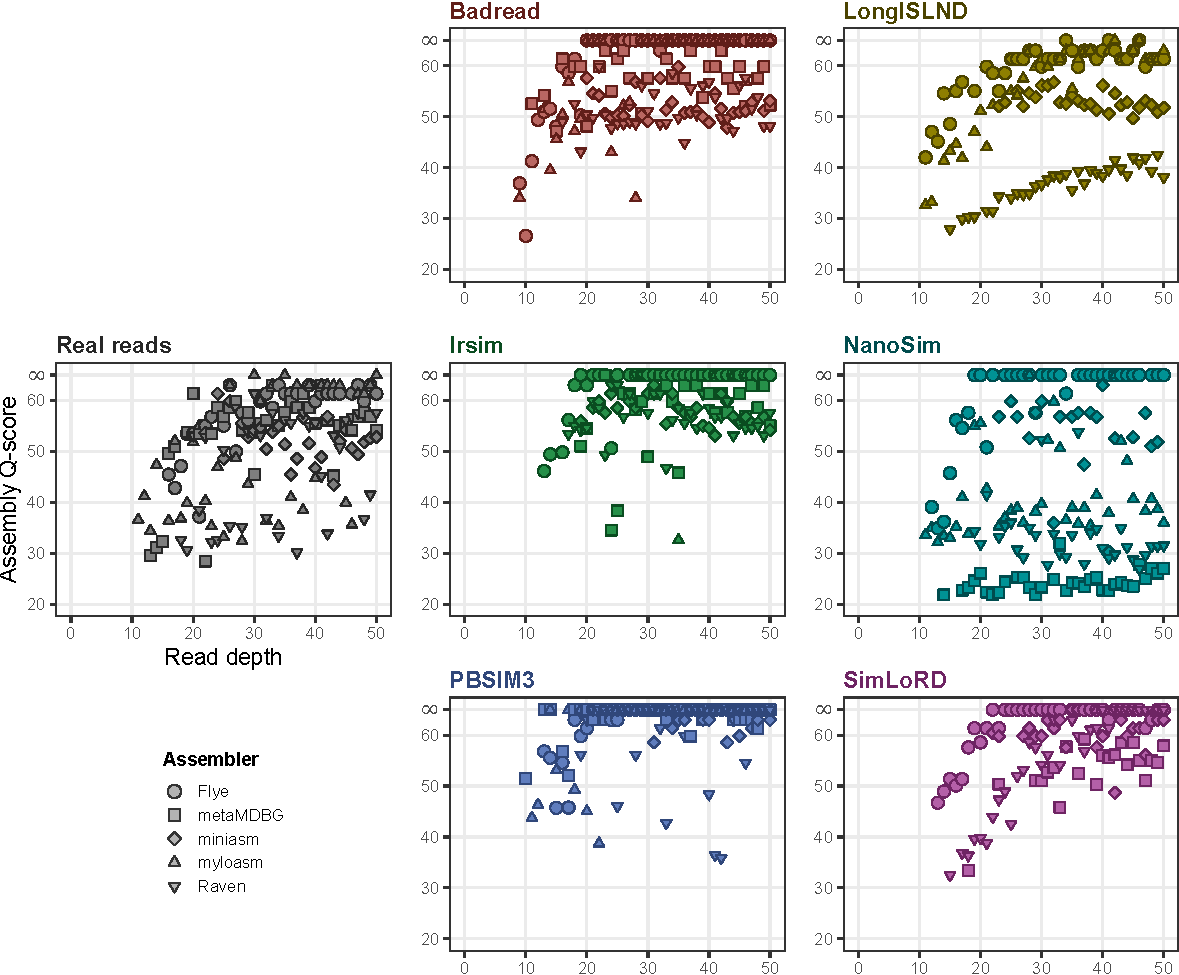
\includegraphics[width=0.69\textwidth]{figure_s7.pdf}
\caption[Assembly accuracy]{\textbf{Assembly accuracy.} For each test read set, we randomly subsampled them to depths ranging from 1--50$\times$. Each subsampled set was assembled with five assemblers: Flye, metaMDBG, miniasm+Minipolish, myloasm and Raven. Assembly accuracy was quantified by taking the longest contig ($\ge$2 Mbp), trimming 1000 bp from each end (to remove assembly artefacts that can arise from non-circular read simulation), aligning to the reference genome and dividing the matching bases by the alignment length. Assemblies were excluded from this plot if their longest contig was shorter than 2 Mbp or if that contig (after trimming) did not produce a single end-to-end alignment. A simulator is more realistic if its plot closely matches that of the real reads.
\par\smallskip
While real reads rarely produced an error-free assembly (Q$\infty$), simulated reads from Badread, lrsim, NanoSim, PBSIM3 and SimLoRD often did, demonstrating that they insufficiently model systematic read errors. LongISLND was best able to mimic the accuracy-vs-depth relationship of the real reads. Some assemblers performed poorly on reads from certain simulators: Raven with LongISLND, metaMDBG with NanoSim, myloasm with NanoSim and Raven with NanoSim.
\par\smallskip
Complete assemblies are drawn as filled points, while incomplete assemblies are drawn as hollow points. An assembly was considered complete if it had exactly two contigs, one with a length matching the chromosome ($\pm$1\%) and the other with a length matching the plasmid ($\pm$1\%). Considering read sets $\ge$20$\times$ depth, real reads produced a complete assembly 61.3\% of the time, Badread 55.5\%, LongISLND 10.3\%, lrsim 22.6\%, NanoSim 14.8\%, PBSIM3 14.8\% and SimLoRD 6.5\%. Of all simulators, only Badread was able to run in a circular-aware mode, i.e. it generated reads that span the start/end junction of the reference sequences. This avoids breaks in read coverage at reference boundaries and likely contributed to its higher assembly completion rate compared with the other tools. While NanoSim does have a similar feature (\texttt{-dna\_type circular}), this does not support reference with multiple sequences, and so it was not usable in this study.
}
\label{fig:supp_assemblies}
\end{figure}


\end{document}
